\documentclass[tikz,dvisvgm,border=1pt]{standalone}
% Shared preamble for the attribution infographics (iN-*.tex).
% tools/tikz-build.sh compiles each source with \variant set to wide or narrow.
\usepackage[T1]{fontenc}
\usepackage[default,semibold]{sourcesanspro}
\usepackage[italic]{mathastext}
% Larger scripts than the TeX default, so subscripts stay legible at phone width.
\DeclareMathSizes{9}{9}{8}{7}
\DeclareMathSizes{10}{10}{9}{8}
\DeclareMathSizes{11}{11}{9}{8}
\DeclareMathSizes{11.5}{11.5}{9.5}{8}
\usetikzlibrary{arrows.meta,positioning,calc,fit,backgrounds,decorations.pathreplacing,patterns}

\ifdefined\variant\else\def\variant{wide}\fi
\newif\ifnarrow
\def\narrowname{narrow}
\ifx\variant\narrowname\narrowtrue\fi
% The narrow variant is about 320pt wide and shown at about 350px, the wide one
% about 540pt wide and shown at up to 720px: the narrow one uses larger type.
\ifnarrow
  \def\basefont{\fontsize{11}{13}\selectfont}\def\smallfont{\fontsize{10}{12}\selectfont}
  \def\titlefont{\fontsize{11.5}{13.5}\selectfont\bfseries}
\else
  \def\basefont{\fontsize{10}{12}\selectfont}\def\smallfont{\fontsize{9}{11}\selectfont}
  \def\titlefont{\fontsize{11}{13}\selectfont\bfseries}
\fi

% Light-theme page tokens (web/src/styles/_variables.css, embeds.css), fixed:
% every infographic sits on its own light card, so it reads on both themes.
\definecolor{ink}{HTML}{262626}      % --text-color on white
\definecolor{muted}{HTML}{666666}    % --muted-color on white
\definecolor{rule}{HTML}{DCDCDC}     % --border-color, slightly stronger
\definecolor{surface}{HTML}{F5F5F5}  % --neutral-200
\definecolor{heading}{HTML}{904B20}  % h2 colour
\definecolor{info}{HTML}{187C9B}     % embeds --info-color
\definecolor{primary}{HTML}{C65928}  % embeds --primary-color
\definecolor{success}{HTML}{35814C}  % embeds --success-color
\definecolor{danger}{HTML}{BD3F50}   % f13 spread cost
\definecolor{residual}{HTML}{A77913} % f13 residual

\tikzset{
  every picture/.style={color=ink, line width=0.6pt, >={Stealth[length=5pt,width=4pt]},
    font=\basefont},
  small/.style={font=\smallfont},
  title/.style={font=\titlefont},
  box/.style={draw=rule, fill=white, rounded corners=4pt, align=center, inner sep=5pt},
  tag/.style={small, text=muted},
}

% No hyphenation in the narrow text columns of the diagrams.
\hyphenpenalty=10000 \exhyphenpenalty=10000

% Light card behind the whole drawing, below the background layer.
\pgfdeclarelayer{card}
\pgfsetlayers{card,background,main}
\newcommand\drawcard{%
  \begin{pgfonlayer}{card}
    \fill[white, draw=rule, rounded corners=8pt]
      ($(current bounding box.south west)+(-10pt,-10pt)$)
      rectangle ($(current bounding box.north east)+(10pt,10pt)$);
  \end{pgfonlayer}}

% Section 3: signals -> construction algorithm -> positions -> P&L, and what each
% attribution method needs. Rerun-based methods (3.1, 3.2, 3.4) sit above the
% pipeline; methods that read the optimiser's equations (3.3) sit below.
\begin{document}
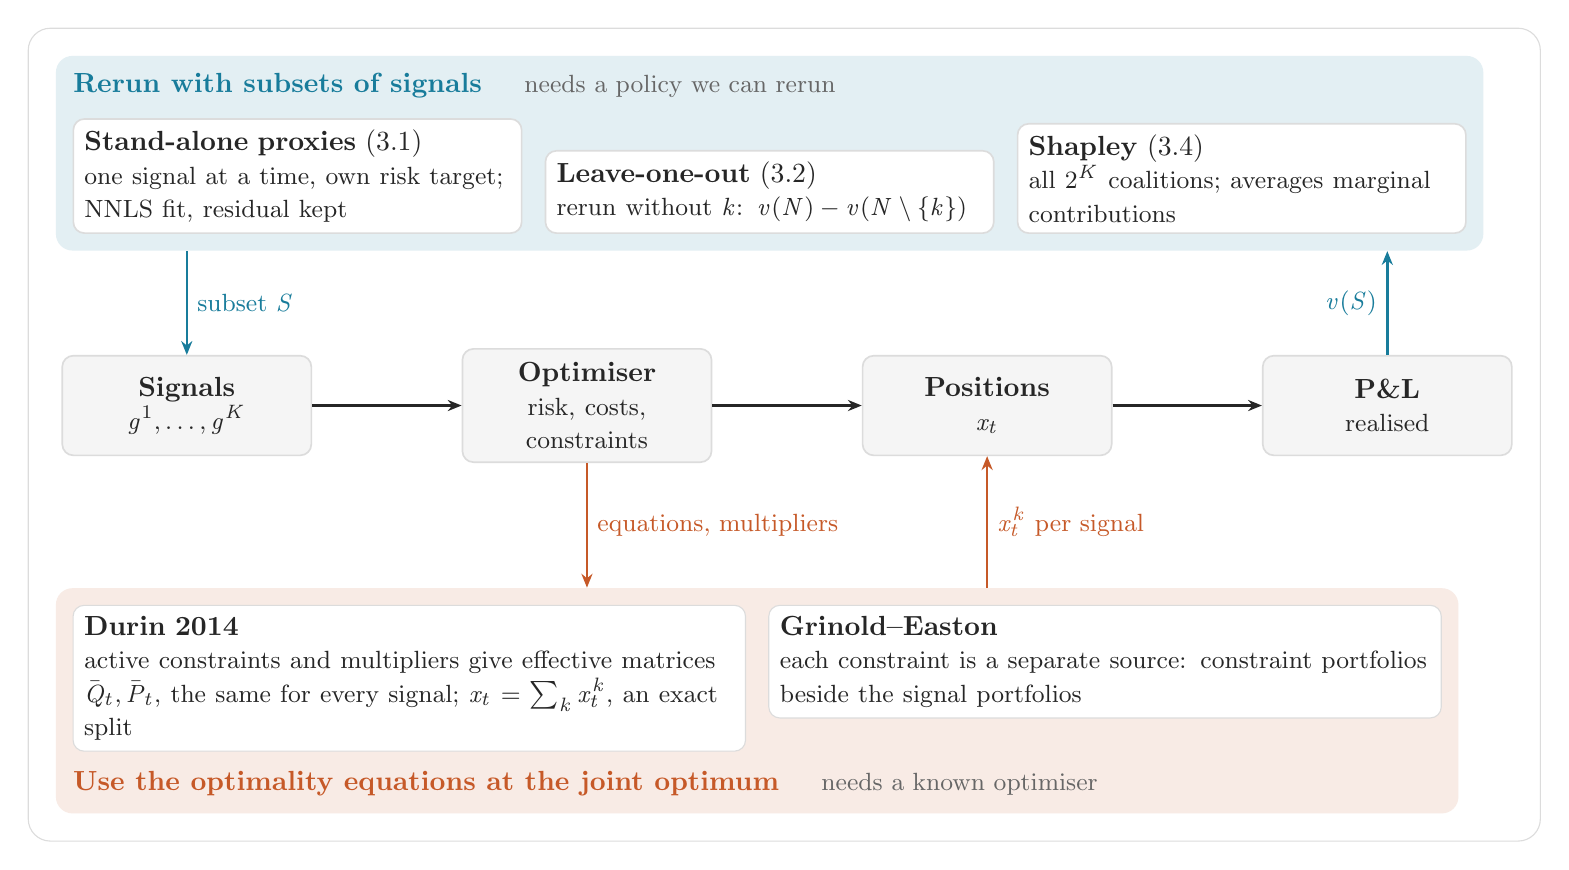
\begin{tikzpicture}[
  stage/.style={box, fill=surface, minimum height=36pt},
  chip/.style={box, align=left, inner sep=4pt},
  band/.style={rounded corners=6pt, inner sep=6pt},
  link/.style={->, line width=0.9pt},
]
\ifnarrow
  \def\W{288pt}\def\chipw{262pt}\def\stagew{48pt}\def\gap{76pt}\def\sep{\\}\def\dlast{d2}
\else
  \def\W{520pt}\def\chipw{154pt}\def\stagew{80pt}\def\gap{144pt}\def\sep{\quad}\def\dlast{d1}
\fi
% Pipeline.
\node[stage, text width=\stagew] (sig) at (0,0) {\textbf{Signals}\\{\smallfont$g^1,\dots,g^K$}};
\node[stage, text width=\stagew, right=\gap-\stagew-10pt of sig] (opt)
  {\textbf{Optimiser}\ifnarrow\else\\{\smallfont risk, costs, constraints}\fi};
\node[stage, text width=\stagew, right=\gap-\stagew-10pt of opt] (pos) {\textbf{Positions}\\{\smallfont$x_t$}};
\node[stage, text width=\stagew, right=\gap-\stagew-10pt of pos] (pnl) {\textbf{P\&L}\\{\smallfont realised}};
\draw[link] (sig) -- (opt); \draw[link] (opt) -- (pos); \draw[link] (pos) -- (pnl);
\ifnarrow
  \node[small, text=muted, below=2pt of opt] (optnote) {risk, costs, constraints};
\fi
\coordinate (L) at ($(sig.west)+(-2pt,0)$);
\coordinate (R) at ($(pnl.east)+(2pt,0)$);

% Rerun-based methods.
\ifnarrow
  \node[chip, text width=\chipw, anchor=south west] (c3) at ($(L)+(0,62pt)$)
    {\textbf{Shapley} (3.4): all $2^K$ coalitions; averages marginal contributions};
  \node[chip, text width=\chipw, above=4pt of c3] (c2)
    {\textbf{Leave-one-out} (3.2): $v(N)-v(N\setminus\{k\})$};
  \node[chip, text width=\chipw, above=4pt of c2] (c1)
    {\textbf{Stand-alone proxies} (3.1): one signal at a time, own risk target; NNLS fit, residual kept};
\else
  \node[chip, text width=\chipw, anchor=south west] (c1) at ($(L)+(6pt,62pt)$)
    {\textbf{Stand-alone proxies} (3.1)\\{\smallfont one signal at a time, own risk target; NNLS fit, residual kept}};
  \node[chip, text width=\chipw, right=8pt of c1.south east, anchor=south west] (c2)
    {\textbf{Leave-one-out} (3.2)\\{\smallfont rerun without $k$: $v(N)-v(N\setminus\{k\})$}};
  \node[chip, text width=\chipw, right=8pt of c2.south east, anchor=south west] (c3)
    {\textbf{Shapley} (3.4)\\{\smallfont all $2^K$ coalitions; averages marginal contributions}};
\fi
\node[anchor=south west, inner sep=0pt, text=info, font=\basefont\bfseries, align=left]
  (rt) at ($(c1.north west)+(0,7pt)$) {Rerun with subsets of signals
  \sep{\smallfont\mdseries\color{muted}needs a policy we can rerun}};
\begin{pgfonlayer}{background}
  \node[band, fill=info!12, fit=(rt)(c1)(c2)(c3)] (rerun) {};
\end{pgfonlayer}
\draw[link, info] (rerun.south -| sig) -- node[right, small] {subset $S$} (sig.north);
\draw[link, info] (pnl.north) -- node[left, small] {$v(S)$} (rerun.south -| pnl);

% Methods that read the optimiser's equations.
\ifnarrow
  \node[chip, text width=\chipw, anchor=north west] (d1) at ($(L)+(0,-74pt)$)
    {\textbf{Durin 2014}: active constraints and multipliers give effective matrices
     $\bar Q_t,\bar P_t$, the same for every signal; $x_t=\sum_k x_t^k$, an exact split};
  \node[chip, text width=\chipw, below=4pt of d1] (d2)
    {\textbf{Grinold--Easton}: each constraint is a separate source; constraint portfolios beside the signal portfolios};
\else
  \node[chip, text width=235pt, anchor=north west] (d1) at ($(L)+(6pt,-72pt)$)
    {\textbf{Durin 2014}\\{\smallfont active constraints and multipliers give effective matrices
     $\bar Q_t,\bar P_t$, the same for every signal; $x_t=\sum_k x_t^k$, an exact split}};
  \node[chip, text width=235pt, right=8pt of d1.north east, anchor=north west] (d2)
    {\textbf{Grinold--Easton}\\{\smallfont each constraint is a separate source: constraint portfolios beside the signal portfolios}};
\fi
\node[anchor=north west, inner sep=0pt, text=primary, font=\basefont\bfseries, align=left]
  (it) at ($(\dlast.south west)+(0,-7pt)$) {Use the optimality equations at the joint optimum
  \sep{\smallfont\mdseries\color{muted}needs a known optimiser}};
\begin{pgfonlayer}{background}
  \node[band, fill=primary!12, fit=(it)(d1)(d2)] (inside) {};
\end{pgfonlayer}
\ifnarrow
  \draw[link, primary] (optnote.south) -- node[right, small, pos=0.45] {equations, multipliers} (inside.north -| opt);
\else
  \draw[link, primary] (opt.south) -- node[right, small] {equations, multipliers} (inside.north -| opt);
  \draw[link, primary] (inside.north -| pos) -- node[right, small] {$x_t^k$ per signal} (pos.south);
\fi
\drawcard
\end{tikzpicture}
\end{document}
